\documentclass[12pt]{report}

\usepackage{geometry}

\usepackage{titlesec}

\setcounter{secnumdepth}{4}

\renewcommand\thesection{\arabic{section}}
\renewcommand\thesubsection{\arabic{section}.\arabic{subsection}}
\renewcommand\thesubsubsection{\arabic{section}.\arabic{subsection}.\arabic{subsubsection}}
\titleformat{\section}
{\normalfont\scshape}{\thesection}{1em}{}
\titleformat{\subsection}
{\normalfont\scshape\small}{\thesubsection}{1em}{}
\titleformat{\subsubsection}
{\normalfont\scshape\small}{\thesubsubsection}{1em}{}

\linespread{1}

\usepackage{cancel}
\usepackage{multirow}

\usepackage{amssymb,amsmath}
\allowdisplaybreaks

\usepackage{xparse}

\usepackage{xtab}

\usepackage [english]{babel}
\usepackage [autostyle, english = american]{csquotes}
\MakeOuterQuote{"}

\usepackage{graphicx}

\usepackage{placeins}

\usepackage{tabularx}
\newcolumntype{L}[1]{>{\raggedright\arraybackslash}p{#1}}
\newcolumntype{C}[1]{>{\centering\arraybackslash}p{#1}}
\newcolumntype{R}[1]{>{\raggedleft\arraybackslash}p{#1}}

\begin{document}
	
	\begin{center}
		\textbf{4-bit CPU Architecture and Assembly.} \\[8pt]
		\small{Keith Allatt} \\
		\small{January 27th, 2019} \\
	\end{center}
	\newpage
	
	\section{CPU Architecture}
	
		\FloatBarrier
	
	\begin{figure}[!hbt]
		\centering
		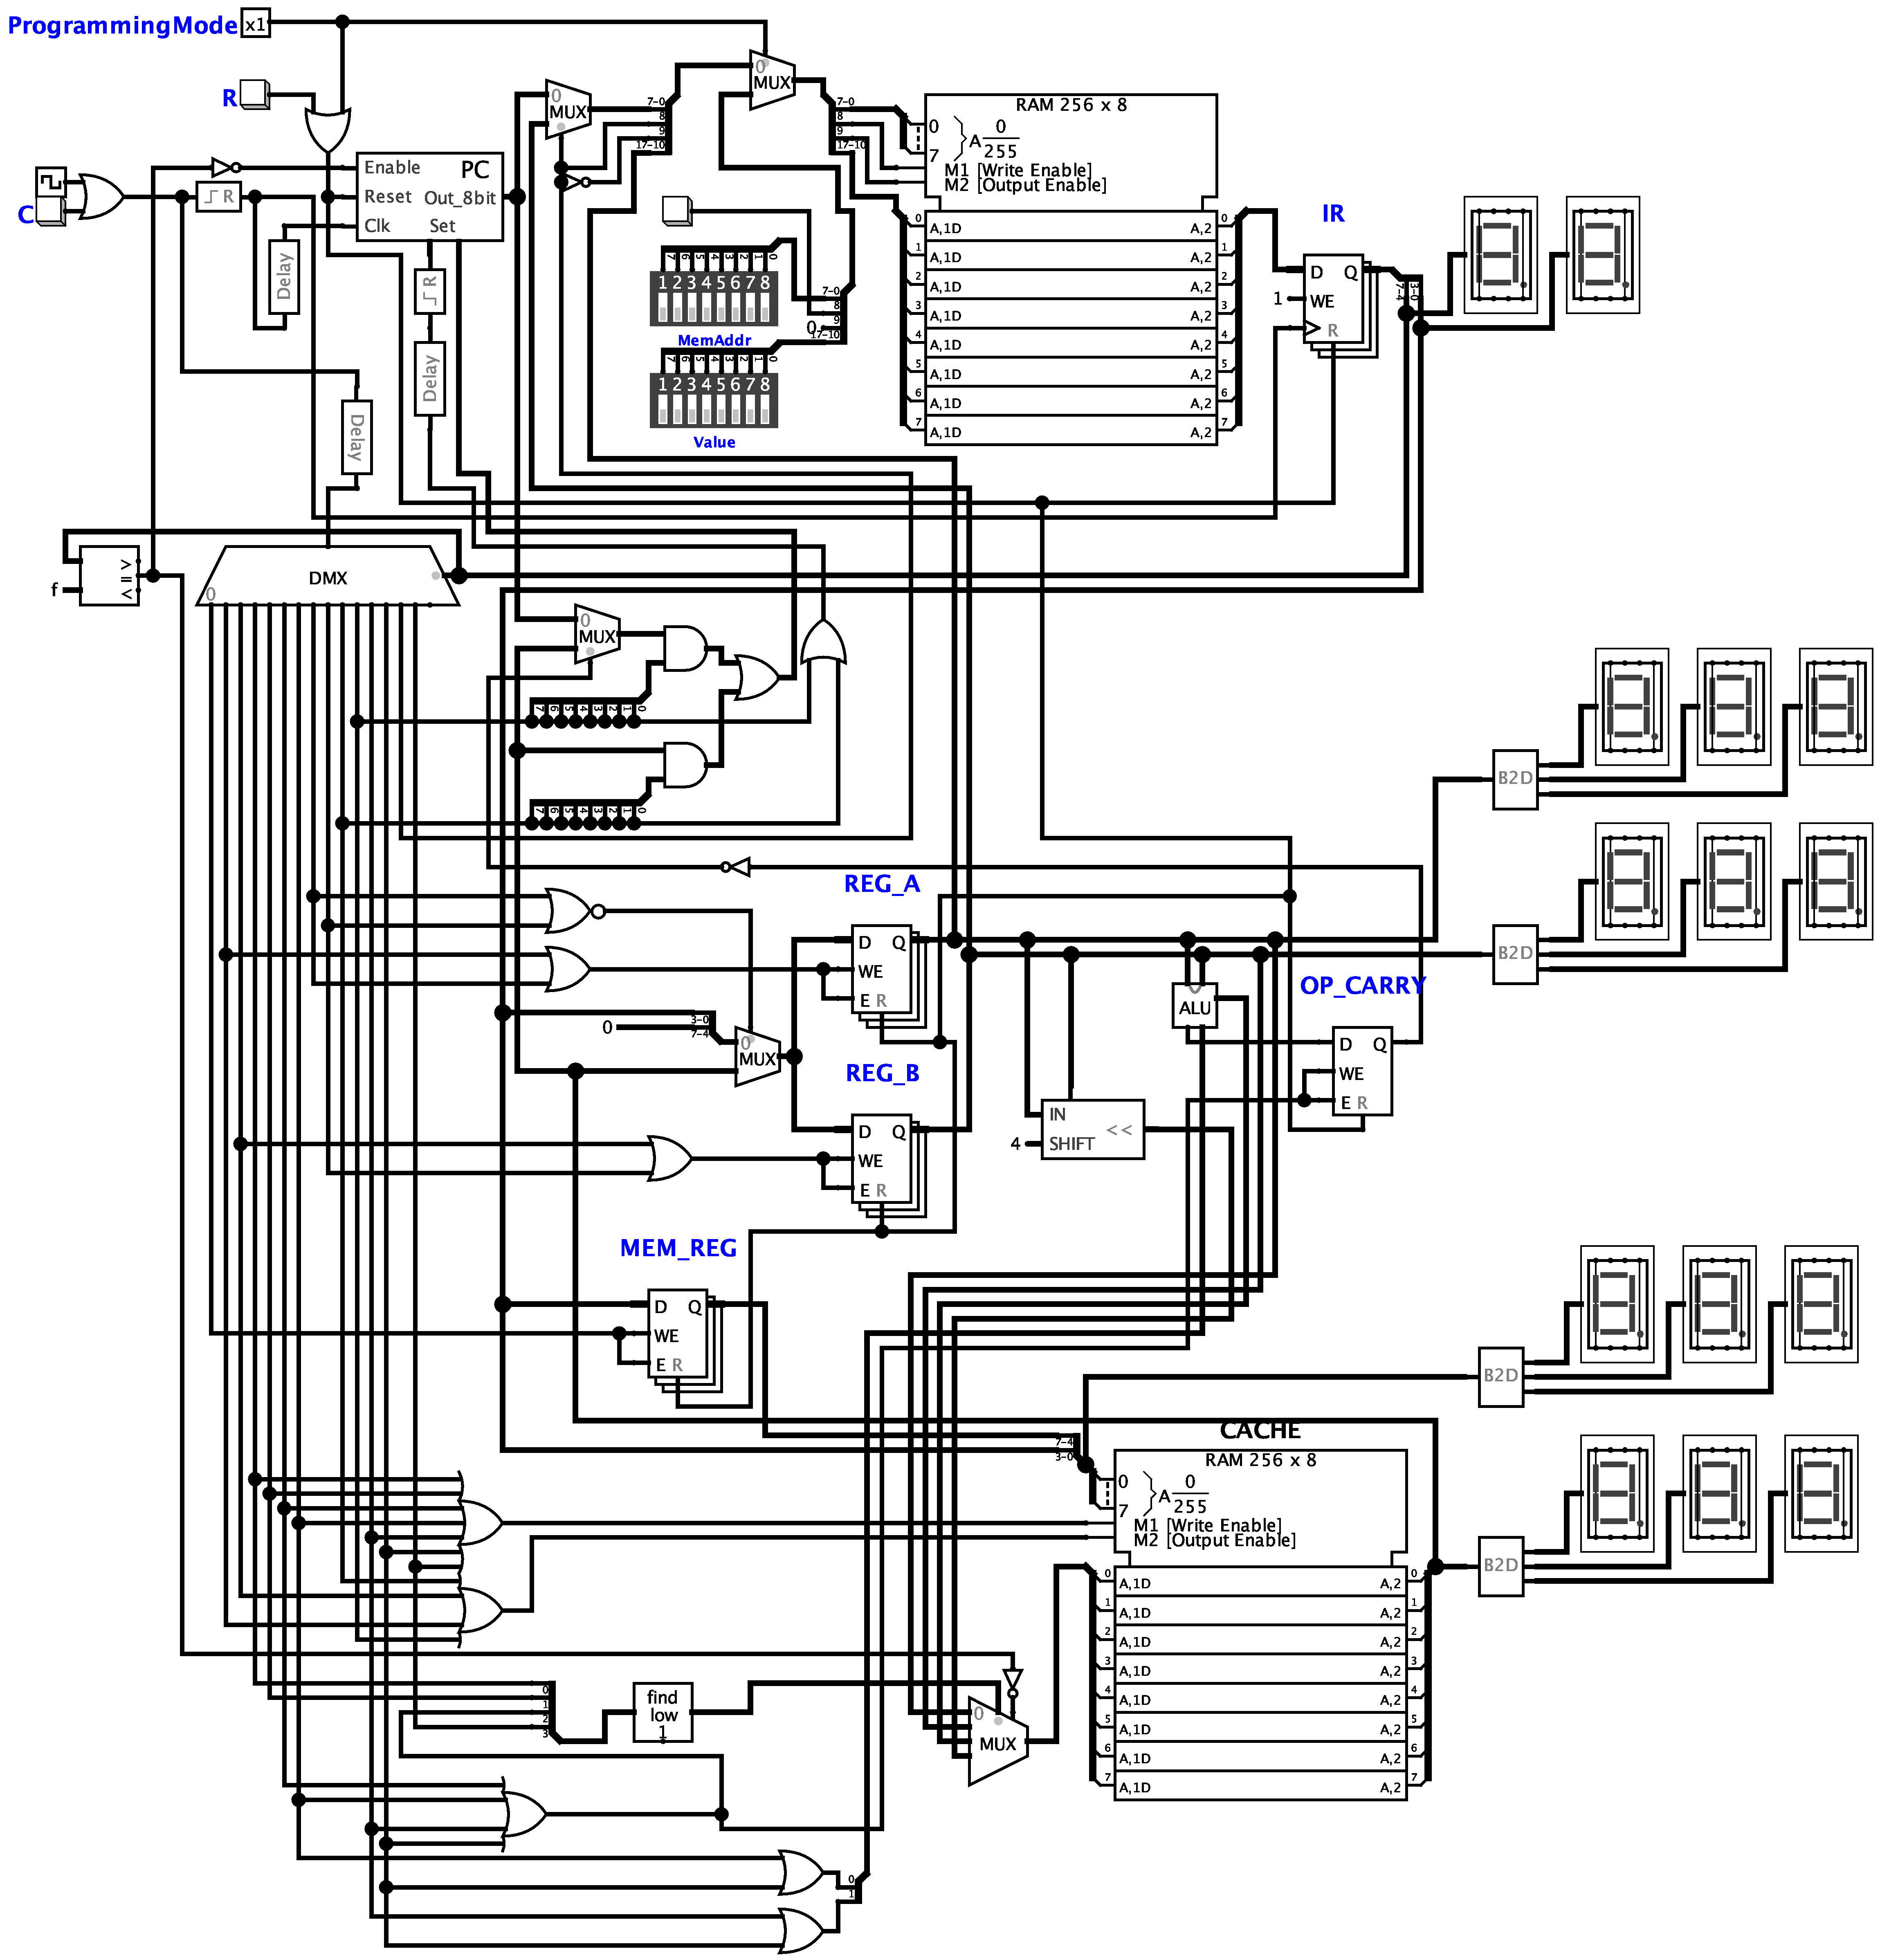
\includegraphics[width=0.75\textwidth]{figures/CPU.png}
		\caption{CPU Architecture}
	\end{figure}

	\begin{figure}[!hbt]
		\centering
		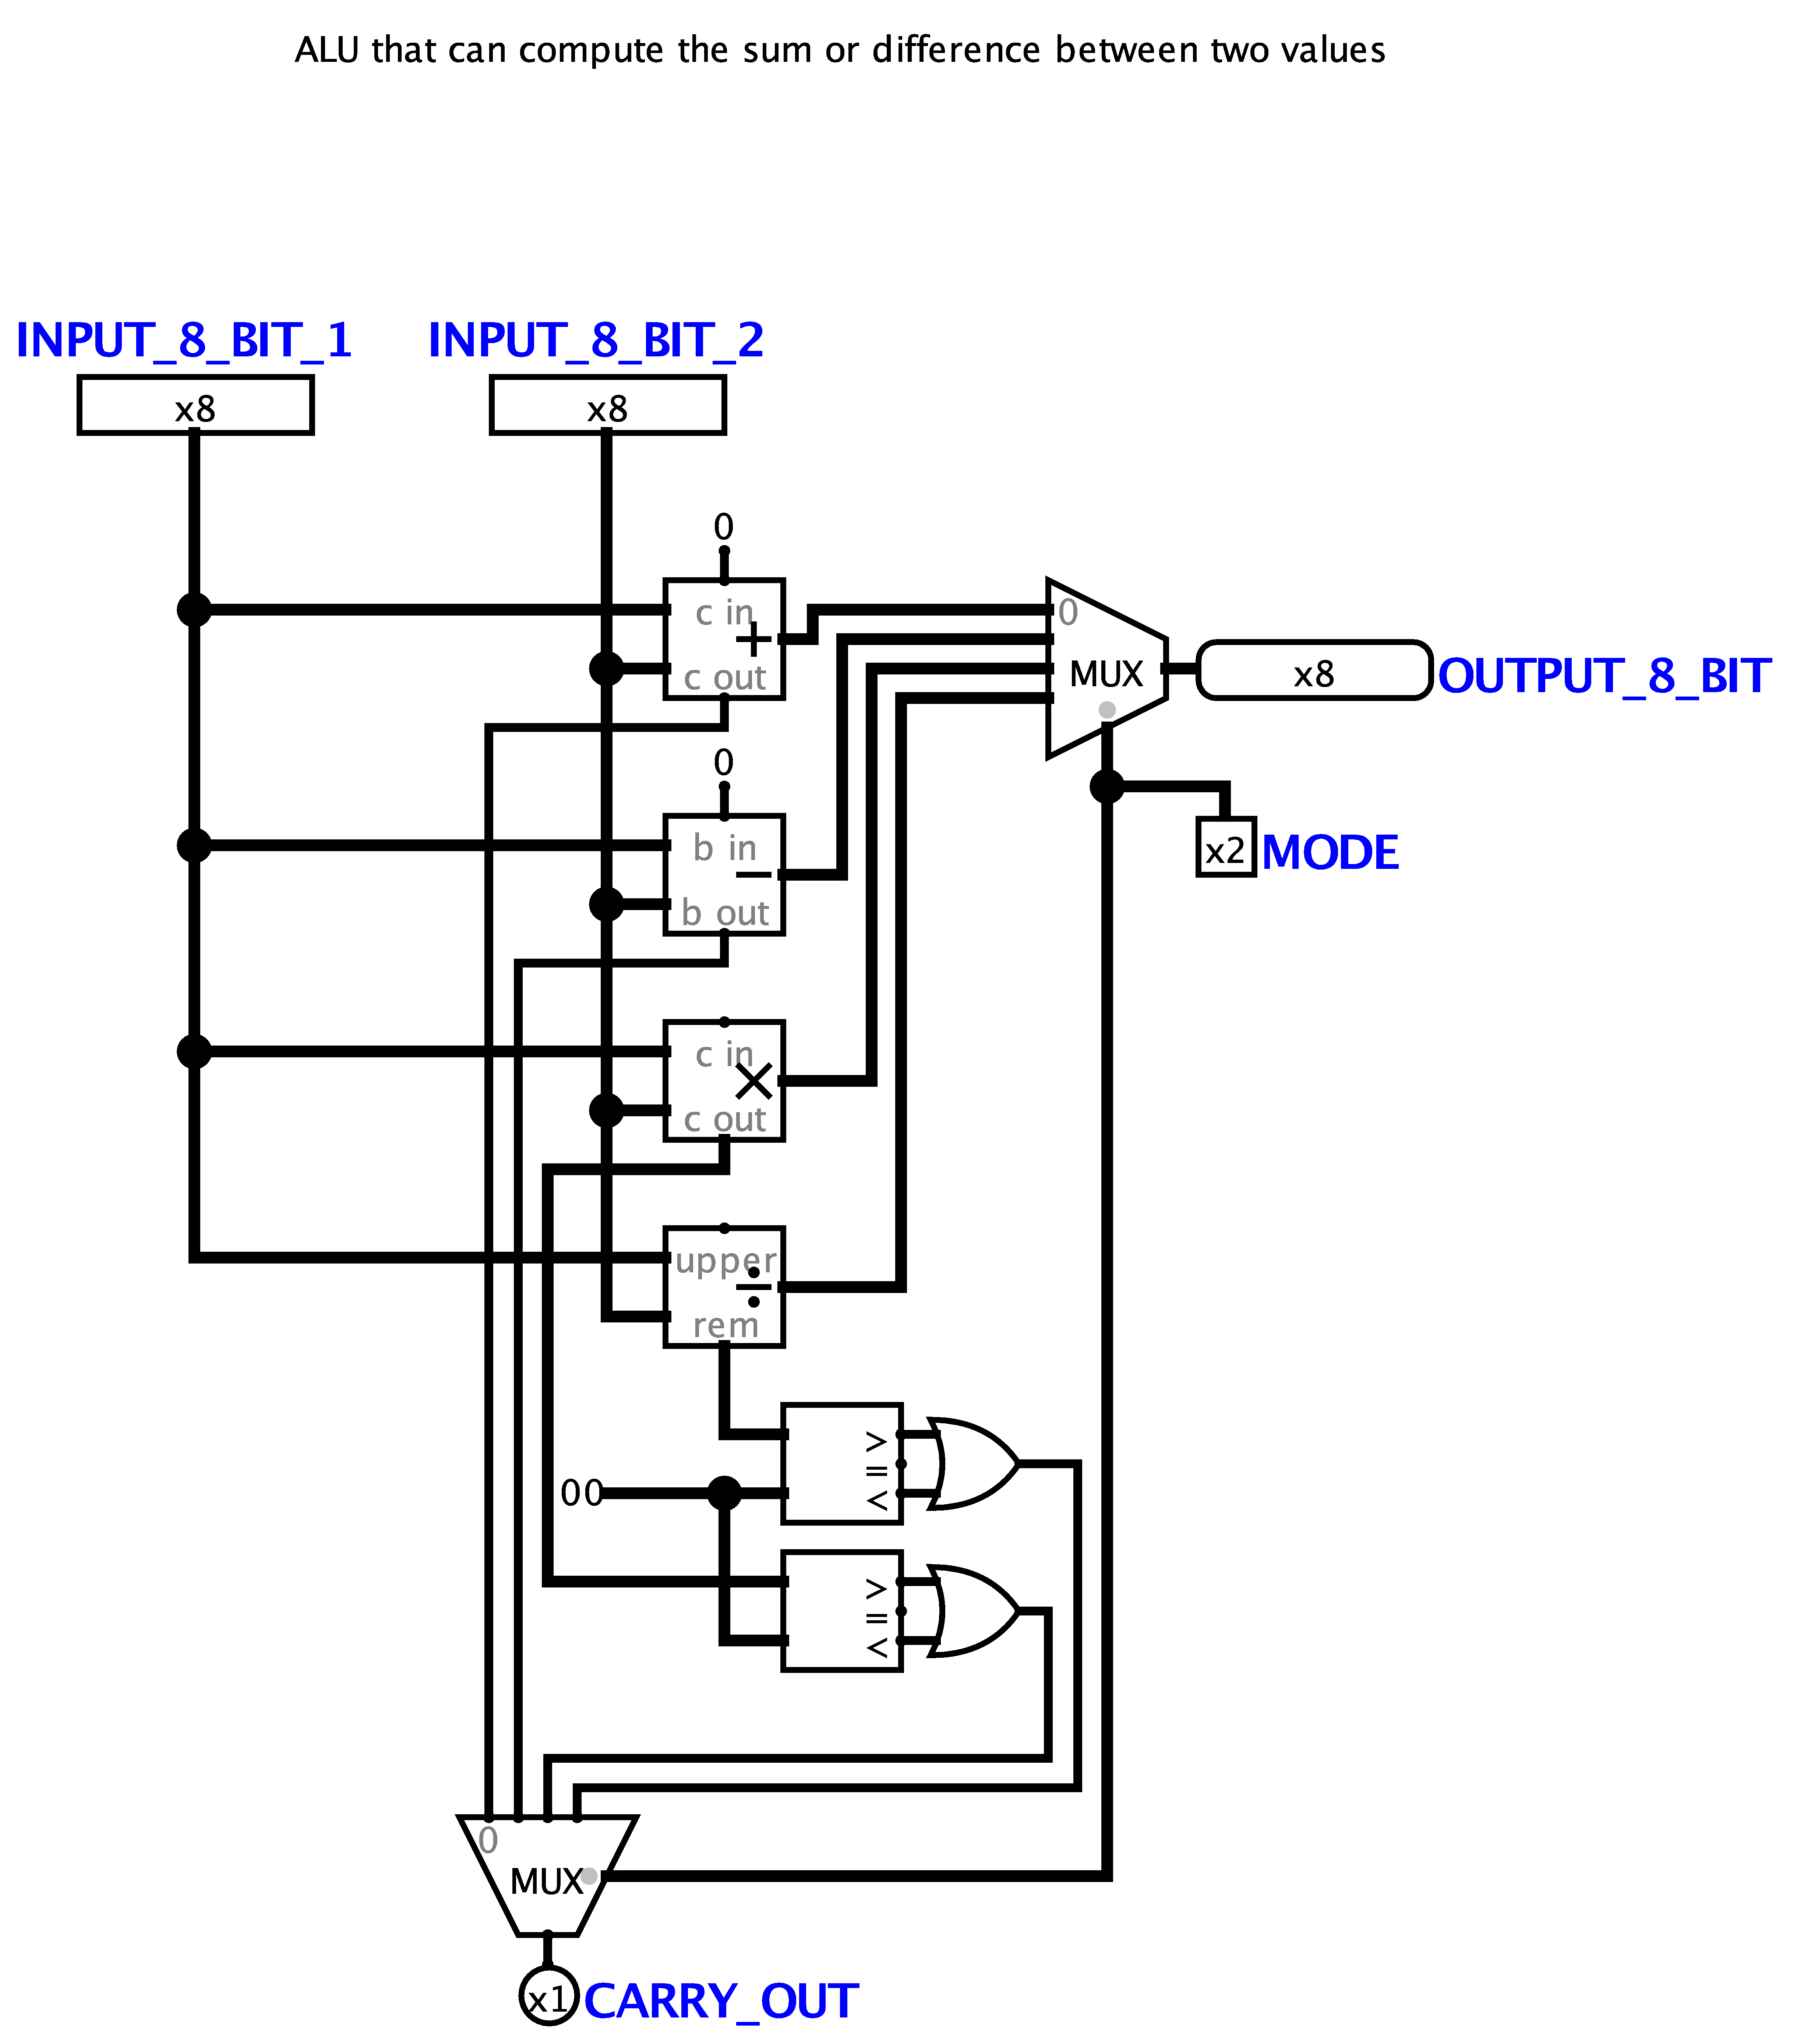
\includegraphics[scale=0.05]{figures/ALU_8_BIT.png}
		\caption{ALU Design}
	\end{figure}

	\begin{figure}[!hbt]
		\centering
		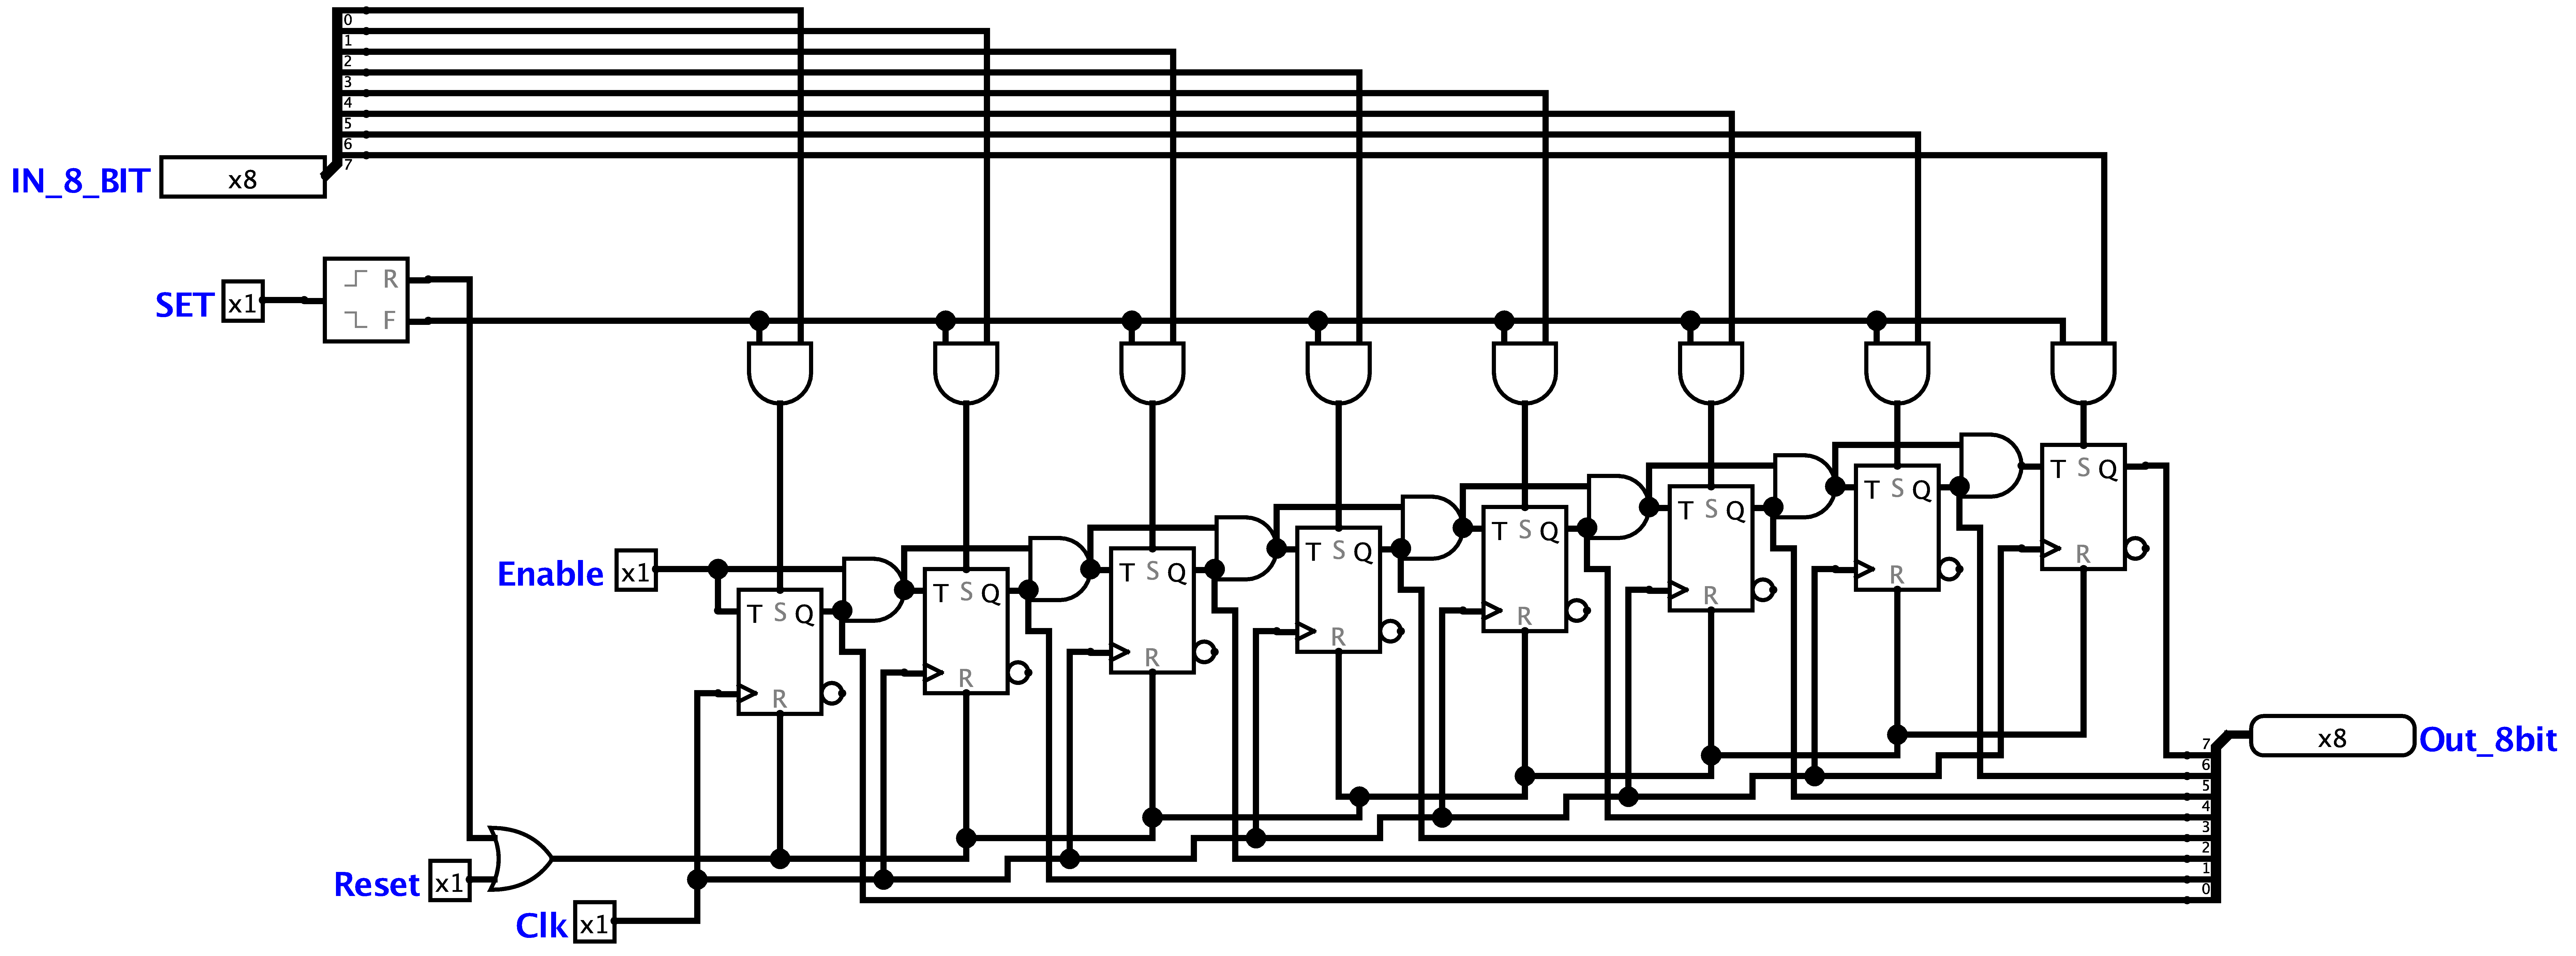
\includegraphics[scale=0.05]{figures/PROG_COUNT.png}
		\caption{Program Counter Design}
	\end{figure}
	
	\FloatBarrier
	
	\begin{itemize}
		\item Can perform addition and subtraction, multiplication and division
		\item Has 2 registers for immediate use
		\item Has 256 bytes of cache memory
		\item Uses a 256 byte RAM instruction list
		\item Programmable
	\end{itemize}

	\FloatBarrier

	

	\section{Assembly}
	
	Each 8-bit assembly command comes in two parts, the Assembly Code, the 4 most significant bits, and the Memory Address, or Mem Addr for short, the 4 least significant bits. Sometimes, the memory address is used as a raw value, and other times it refers to a memory address in cache.	\
	
	\FloatBarrier
	\begin{table}[!hbt]
		\centering
		\begin{tabular}{|l|l|l|l|l|}
			\hline
			Code 	& Name 		& Function 								& Input 	& Output 	\\ \hline
			0		& SET MEM	& Set the 4 MSBs of the mem addr		& Mem Addr	& Mem Reg 	\\ \hline
			1 		& LOAD A 	& Load from cache into Register A		& Cache 	& Reg A		\\ \hline
			2 		& LOAD B 	& Load from cache into Register B		& Cache 	& Reg B		\\ \hline
			3 		& WRITE A	& Write to cache from Register A		& Reg A 	& Cache		\\ \hline
			4 		& WRITE B	& Write to cache from Register B		& Reg B		& Cache		\\ \hline
			5 		& ADD A B	& Write A+B to cache					& Reg A, B	& Cache		\\ \hline
			6 		& SUB A B	& Write A-B to cache 					& Reg A, B	& Cache		\\ \hline
			7 		& SET A		& Set the value in Register A			& Mem Addr	& N/a		\\ \hline
			8 		& SET B		& Set the value in Register B			& Mem Addr	& N/a		\\ \hline
			9 		& NC JUMP	& Jump to line 							& Mem Addr	& N/a		\\ \hline
			a 		& C JUMP	& Jump if carry bit is 0, cont. when 1	& Mem Addr	& N/a		\\ \hline
			b 		& MUL A B	& Write A$\times$B to cache				& Reg A, B	& Cache		\\ \hline
			c 		& DIV A B	& Write A$\div$B to cache 				& Reg A, B	& Cache		\\ \hline
			d		& MOD IR	& Write Reg A to a IR at MA in Reg B	& N/a		& IR		\\ \hline
			e 		& LS REG	& Write A $<<$ 4 + B to cache			& N/a		& Cache		\\ \hline
			f 		& HALT		& Program Halts							& N/a		& N/a		\\ \hline
		\end{tabular}
	\end{table}
	\FloatBarrier

	\subsection{Simple Operations and Programs}
	
	Many simple tasks don't require changing memory address pages but many do as well. Here are some simpler code snippets.
	
	\subsubsection{Clearing a page of Cache}
	
	In this context, a page of cache refers to a 16 byte chunk of memory where the 4 most significant bits remain constant. For example, a memory addresses in the 0th page would be somewhere in the range 00 to 0f, the 2nd page in the range 20 to 2f, the last page somewhere in the range f0 to ff.
	
	\FloatBarrier
	\begin{table}[!ht]
		\begin{tabular}{lll}
			Code 			& Name 				& Description \\ \hline
			70 				& SET A 			& Set Reg A to 0 \\
			30 				& WRITE A 			& Write A, which is 0, into cache at mem. addr. 0 \\
			31 				& WRITE A 			& Write A, which is 0, into cache at mem. addr. 1 \\
			32 				& WRITE A 			& Write A, which is 0, into cache at mem. addr. 2 \\
			$\vdots$		& $\vdots$			& $\vdots$ \\
			3e 				& WRITE A 			& Write A, which is 0, into cache at mem. addr. e \\
			3f	 			& WRITE A			& Write A, which is 0, into cache at mem. addr. f \\
			ff				& HALT				& Program is done. Cache is cleared. \\
		\end{tabular}
	\end{table}
	\FloatBarrier
	
	
	
	\subsubsection{Putting an 8-bit number into a register}
	
	For arguments sake, let us be putting an 8-bit number into register A, and let mem. addr. 0 in the cache be free. If not, replace the calls to mem. addr. 0 with the mem. addr. that's free.
	
	Let the number being inputted be represented as XY where X and Y are hexadecimal digits.
	
	\FloatBarrier
	\begin{table}[!ht]
		\begin{tabular}{lll}
			Code 			& Name 				& Description \\ \hline
			7X 				& SET A 			& Set Reg A to X \\
			8Y 				& SET B 			& Set Reg B to Y \\
			e0 				& LS REG 			& Left shift Reg A by 4 places and add B, store in mem. addr. 0 \\
			10				& LOAD A			& Load the value XY in mem. addr. 0 to Reg A \\
			80				& SET B				& Set Reg B to 0 \\
			40				& WRITE B			& Write the contents of B, the value 0, to the cache at mem. addr. 0 \\
			ff				& HALT				& Program is done. The value XY is in Reg A \\
		\end{tabular}
	\end{table}
	\FloatBarrier
	
	\subsubsection{Switching Registers}
	
	For arguments sake, let the mem. addr.'s 0 and 1 be free.
		
	\FloatBarrier
	\begin{table}[!ht]
		\begin{tabular}{lll}
			Code 			& Name 				& Description \\ \hline
			30				& WRITE A			& Write Reg A to mem. addr. 0 \\	
			41				& WRITE B			& Write Reg B to mem. addr. 1 \\	
			11				& LOAD A			& Load Reg A from mem. addr. 1 \\	
			20				& LOAD B			& Load Reg B from mem. addr. 0 \\	
		\end{tabular}
	\end{table}
	\FloatBarrier
	
\end{document}
